\documentclass[12pt,a4paper]{article}

% Packages
\usepackage[utf8]{inputenc}
\usepackage[margin=1in]{geometry}
\usepackage{graphicx}
\usepackage{hyperref}
\usepackage{xcolor}
\usepackage{amsmath}
\usepackage{amssymb}
\usepackage{tikz}
\usepackage{enumitem}
\usepackage{tcolorbox}
\usepackage{fancyhdr}
\usepackage{tabularx}

% TikZ libraries
\usetikzlibrary{shapes.geometric, arrows, positioning, fit, backgrounds, shadows}

% Custom colors
\definecolor{switchitblue}{RGB}{41, 128, 185}
\definecolor{switchitgreen}{RGB}{39, 174, 96}
\definecolor{switchitorange}{RGB}{230, 126, 34}
\definecolor{switchitpurple}{RGB}{142, 68, 173}
\definecolor{switchitred}{RGB}{231, 76, 60}

% Header and footer
\pagestyle{fancy}
\fancyhf{}
\rhead{SwitchIt Companion AI}
\lhead{Implementation Plan}
\rfoot{Page \thepage}

\title{\Huge\textbf{SwitchIt Companion AI} \\ \Large Implementation Plan \& Integration Roadmap}
\author{SwitchIt Technical Team}
\date{\today}

\begin{document}

\maketitle
\tableofcontents
\newpage

%===========================================
\section{Executive Summary}
%===========================================

\subsection{What is SwitchIt Companion AI?}

The \textbf{SwitchIt Companion AI} is an intelligent, persistent mentor built directly into the SwitchIt platform. Unlike typical chatbots that forget conversations after you close them, this AI companion:

\begin{itemize}[leftmargin=*]
    \item \textbf{Remembers You:} Tracks your career goals, achievements, setbacks, and progress over months and years
    \item \textbf{Understands Context:} Knows what you're working on within SwitchIt (job applications, posts, connections)
    \item \textbf{Guides Growth:} Provides personalized advice for professional and personal development
    \item \textbf{Adapts to You:} Adjusts its teaching style based on your emotional state and learning patterns
    \item \textbf{Teaches Actively:} Creates quizzes, challenges, and learning plans tailored to your career path
\end{itemize}

\begin{tcolorbox}[colback=switchitblue!10,colframe=switchitblue,title=\textbf{The Big Idea}]
\large
\textit{LinkedIn asks: "Who are you?"}

\vspace{0.3cm}
\textit{SwitchIt asks: "Who are you becoming?"}

\vspace{0.3cm}
The AI Companion is your personal narrator on that journey of transformation.
\end{tcolorbox}

\subsection{Why This Matters}

\paragraph{For Users:}
\begin{itemize}
    \item Get personalized career guidance 24/7
    \item Track progress toward professional goals
    \item Learn new skills through interactive challenges
    \item Receive emotional support during job search struggles
    \item Feel motivated and accountable
\end{itemize}

\paragraph{For SwitchIt:}
\begin{itemize}
    \item \textbf{Differentiation:} Stand out from LinkedIn with a truly innovative feature
    \item \textbf{Engagement:} Keep users coming back daily to interact with their companion
    \item \textbf{Retention:} Users invested in their growth journey stay longer
    \item \textbf{Data Intelligence:} Better understand user needs and career trajectories
    \item \textbf{Network Effects:} Successful users become advocates for the platform
\end{itemize}

\subsection{Vision Statement}

\begin{center}
\fcolorbox{switchitpurple}{switchitpurple!5}{%
\parbox{0.9\textwidth}{%
\centering
\large
\textit{"To transform SwitchIt from a static professional profile platform into a dynamic growth platform where every user has a personal AI mentor guiding their career journey, making professional success more accessible and personalized."}
}
}
\end{center}

%===========================================
\section{How It Works: The User Experience}
%===========================================

\subsection{User Journey Overview}

\begin{center}
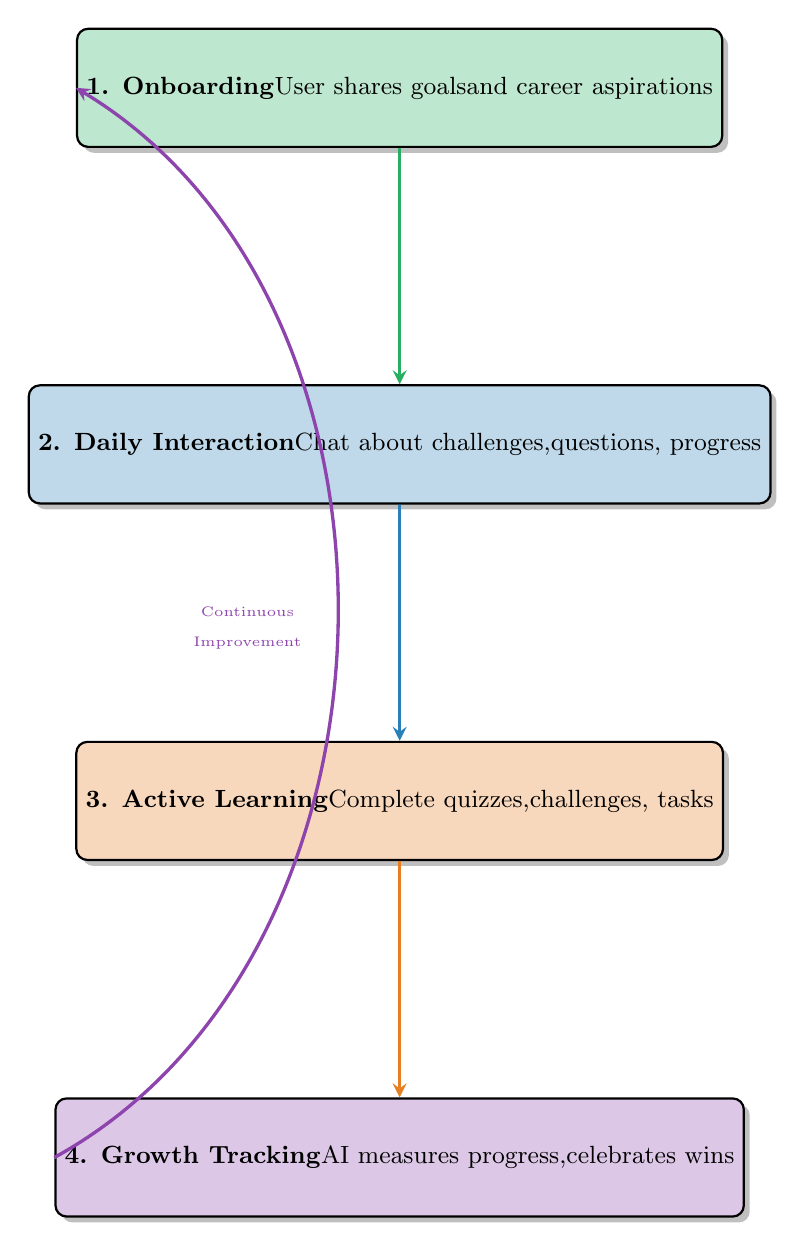
\begin{tikzpicture}[
    node distance=3cm,
    every node/.style={font=\small},
    box/.style={rectangle, rounded corners, minimum width=4cm, minimum height=1.5cm, text centered, draw=black, line width=0.8pt, drop shadow},
    arrow/.style={->, >=stealth, line width=1.2pt}
]

\node[box, fill=switchitgreen!30] (onboard) {
    \textbf{1. Onboarding}\\
    User shares goals\\
    and career aspirations
};

\node[box, fill=switchitblue!30, below=of onboard] (chat) {
    \textbf{2. Daily Interaction}\\
    Chat about challenges,\\
    questions, progress
};

\node[box, fill=switchitorange!30, below=of chat] (learn) {
    \textbf{3. Active Learning}\\
    Complete quizzes,\\
    challenges, tasks
};

\node[box, fill=switchitpurple!30, below=of learn] (grow) {
    \textbf{4. Growth Tracking}\\
    AI measures progress,\\
    celebrates wins
};

\draw[arrow, switchitgreen] (onboard) -- (chat);
\draw[arrow, switchitblue] (chat) -- (learn);
\draw[arrow, switchitorange] (learn) -- (grow);
\draw[arrow, switchitpurple, bend right=60] (grow.west) to node[left, text width=2cm, align=center] {\tiny Continuous\\Improvement} (onboard.west);

\end{tikzpicture}
\end{center}

\subsection{Example Scenarios}

\subsubsection{Scenario 1: Job Seeker Struggling with Interviews}

\begin{enumerate}[leftmargin=*]
    \item \textbf{User shares:} "I had another interview rejection today. I don't know what I'm doing wrong."
    
    \item \textbf{AI responds empathetically:} Acknowledges the disappointment and asks about the interview details
    
    \item \textbf{AI analyzes:} Reviews user's past interview experiences stored in memory
    
    \item \textbf{AI creates action plan:}
    \begin{itemize}
        \item Identifies pattern: User struggles with system design questions
        \item Generates personalized 5-day learning plan
        \item Creates practice quizzes on system design
        \item Schedules daily check-ins
    \end{itemize}
    
    \item \textbf{AI follows up:} Tracks completion of learning tasks and adjusts difficulty
    
    \item \textbf{Next interview:} AI sends motivational message and key reminders
    
    \item \textbf{After success:} Celebrates achievement and updates user's skill profile
\end{enumerate}

\subsubsection{Scenario 2: Early Career Professional Seeking Direction}

\begin{enumerate}[leftmargin=*]
    \item \textbf{User asks:} "Should I focus on frontend or backend development?"
    
    \item \textbf{AI reviews:} User's SwitchIt posts, projects, endorsements, and interests
    
    \item \textbf{AI identifies:} User has more engagement with frontend content
    
    \item \textbf{AI suggests:} Personalized path with specific milestones
    
    \item \textbf{AI creates:} Learning roadmap with weekly goals
    
    \item \textbf{AI monitors:} User's progress through SwitchIt activity (posts about frontend projects)
    
    \item \textbf{AI adjusts:} Recommendations based on what's working vs. what's not
\end{enumerate}

\subsection{Key Features from User Perspective}

\begin{table}[h]
\centering
\begin{tabularx}{\textwidth}{|l|X|}
\hline
\textbf{Feature} & \textbf{User Benefit} \\
\hline
\textbf{Persistent Memory} & AI remembers your entire career journey—never repeat yourself \\
\hline
\textbf{Goal Tracking} & Set and monitor career goals with AI accountability \\
\hline
\textbf{Adaptive Learning} & Get quizzes and challenges that match your current skill level \\
\hline
\textbf{Emotional Intelligence} & Receive empathy during setbacks, motivation during plateaus \\
\hline
\textbf{Platform Integration} & AI automatically knows what you're doing on SwitchIt \\
\hline
\textbf{Proactive Nudges} & Get reminders and suggestions when you need them most \\
\hline
\textbf{Progress Dashboard} & Visualize your growth over time with clear metrics \\
\hline
\end{tabularx}
\caption{User-Facing Features and Benefits}
\end{table}

%===========================================
\section{System Architecture: Simplified Overview}
%===========================================

\subsection{The Three Core Components}

Think of the SwitchIt Companion AI as having three main "brains" that work together:

\begin{center}
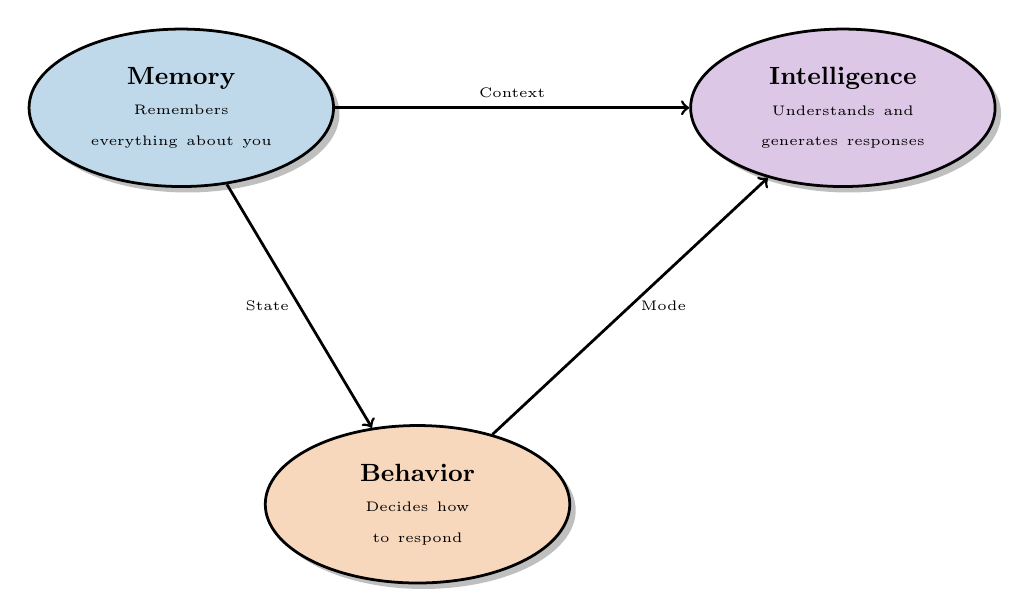
\begin{tikzpicture}[
    node distance=2.5cm,
    every node/.style={font=\small},
    brain/.style={ellipse, minimum width=3cm, minimum height=2cm, text centered, draw=black, line width=1pt, drop shadow, text width=2.5cm}
]

\node[brain, fill=switchitblue!30] (memory) {
    \textbf{Memory}\\
    \tiny Remembers everything about you
};

\node[brain, fill=switchitpurple!30, right=of memory, xshift=2cm] (intelligence) {
    \textbf{Intelligence}\\
    \tiny Understands and generates responses
};

\node[brain, fill=switchitorange!30, below=of memory, yshift=-0.5cm, xshift=3cm] (behavior) {
    \textbf{Behavior}\\
    \tiny Decides how to respond
};

\draw[->, line width=1pt] (memory) -- node[above, font=\tiny] {Context} (intelligence);
\draw[->, line width=1pt] (behavior) -- node[right, font=\tiny] {Mode} (intelligence);
\draw[->, line width=1pt] (memory) -- node[left, font=\tiny] {State} (behavior);

\end{tikzpicture}
\end{center}

\paragraph{1. Memory Brain:}
\begin{itemize}
    \item Stores all your conversations, goals, achievements, and failures
    \item Recalls relevant information when you chat
    \item Tracks patterns in your behavior and progress
    \item Connects to your SwitchIt profile, posts, and activity
\end{itemize}

\paragraph{2. Intelligence Brain:}
\begin{itemize}
    \item Uses advanced AI (like ChatGPT) to understand your messages
    \item Generates personalized, thoughtful responses
    \item Creates learning content (quizzes, plans, challenges)
    \item Analyzes your emotional state from what you write
\end{itemize}

\paragraph{3. Behavior Brain:}
\begin{itemize}
    \item Decides \textit{how} the AI should respond to you
    \item Chooses between empathy, motivation, teaching, or challenging
    \item Adjusts difficulty of tasks based on your current state
    \item Determines when to be proactive vs. reactive
\end{itemize}

\subsection{High-Level Data Flow}

\begin{center}
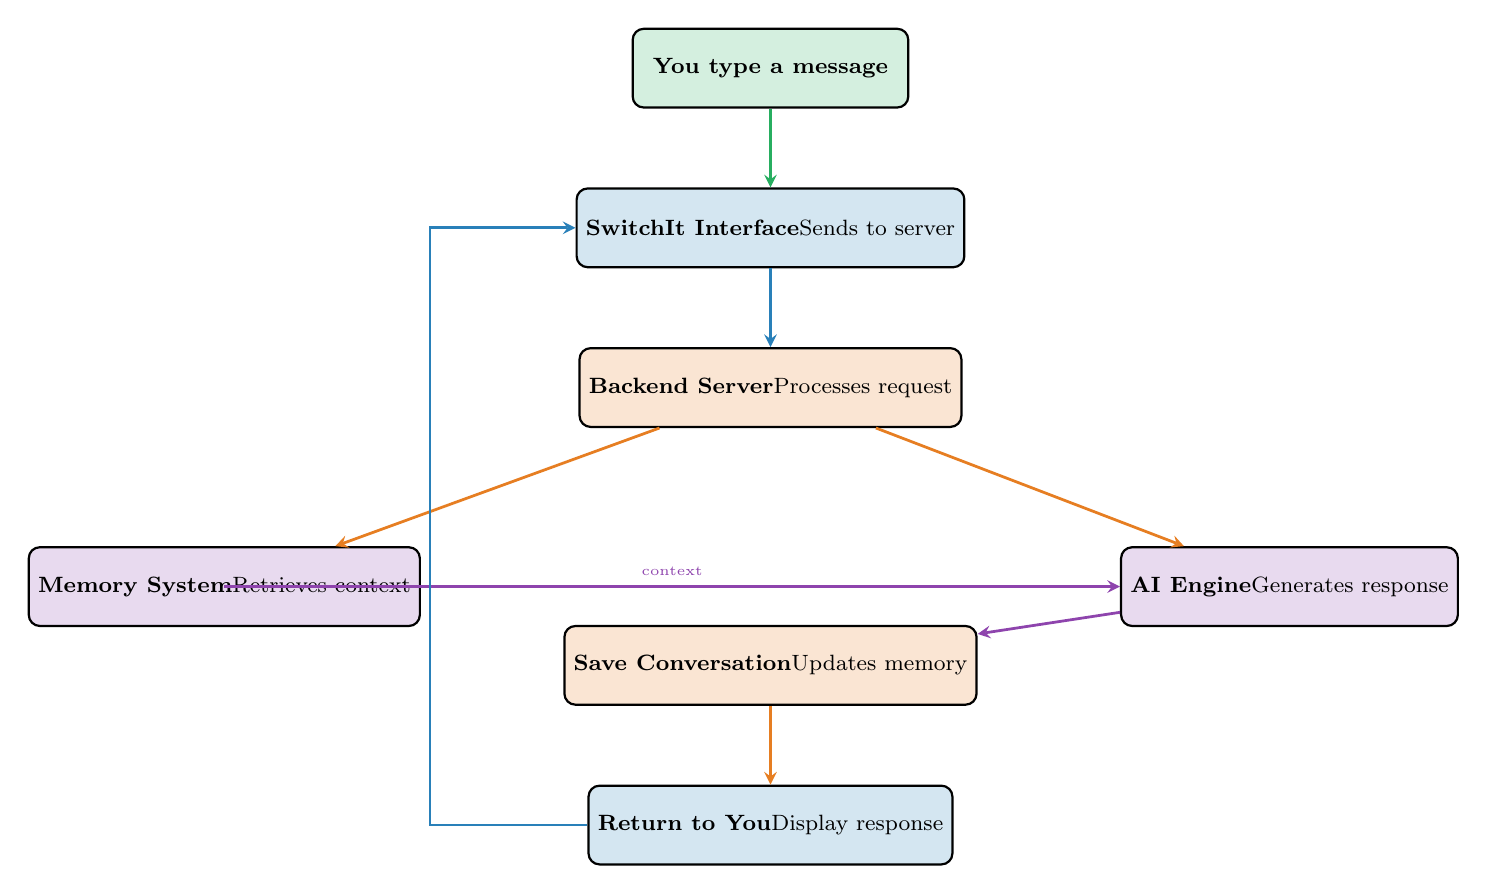
\begin{tikzpicture}[
    node distance=1.5cm,
    every node/.style={font=\footnotesize},
    component/.style={rectangle, rounded corners, minimum width=3.5cm, minimum height=1cm, text centered, draw=black, fill=white, line width=0.8pt},
    arrow/.style={->, >=stealth, line width=1pt}
]

\node[component, fill=switchitgreen!20] (user) {\textbf{You type a message}};

\node[component, fill=switchitblue!20, below=1cm of user] (frontend) {\textbf{SwitchIt Interface}\\Sends to server};

\node[component, fill=switchitorange!20, below=1cm of frontend] (server) {\textbf{Backend Server}\\Processes request};

\node[component, fill=switchitpurple!20, below left=1.5cm and 2cm of server] (memory) {\textbf{Memory System}\\Retrieves context};

\node[component, fill=switchitpurple!20, below right=1.5cm and 2cm of server] (ai) {\textbf{AI Engine}\\Generates response};

\node[component, fill=switchitorange!20, below=2.5cm of server] (save) {\textbf{Save Conversation}\\Updates memory};

\node[component, fill=switchitblue!20, below=1cm of save] (return) {\textbf{Return to You}\\Display response};

\draw[arrow, color=switchitgreen] (user) -- (frontend);
\draw[arrow, color=switchitblue] (frontend) -- (server);
\draw[arrow, color=switchitorange] (server) -- (memory);
\draw[arrow, color=switchitorange] (server) -- (ai);
\draw[arrow, color=switchitpurple] (memory) |- node[above, near end] {\tiny context} (ai);
\draw[arrow, color=switchitpurple] (ai) -- (save);
\draw[arrow, color=switchitorange] (save) -- (return);
\draw[arrow, color=switchitblue] (return.west) -- ++(-2,0) |- (frontend.west);

\end{tikzpicture}
\end{center}

\subsection{Technology Components Explained}

\begin{table}[h]
\centering
\begin{tabularx}{\textwidth}{|l|X|X|}
\hline
\textbf{Component} & \textbf{What It Does} & \textbf{Why We Need It} \\
\hline
\textbf{Frontend (React)} & The chat interface you see & Beautiful, interactive user experience \\
\hline
\textbf{Backend Server} & Manages all requests & Coordinates between components securely \\
\hline
\textbf{AI Model (GPT-4)} & Understands \& generates text & Powers natural conversation \\
\hline
\textbf{Vector Database} & Stores conversation memories & Fast semantic search of past chats \\
\hline
\textbf{SQL Database} & Stores structured data & Goals, events, user profiles \\
\hline
\textbf{Cache (Redis)} & Temporary quick storage & Faster response times \\
\hline
\end{tabularx}
\caption{Technology Stack Explained Simply}
\end{table}

%===========================================
\section{Implementation Roadmap}
%===========================================

\begin{tcolorbox}[colback=yellow!10,colframe=orange,title=\textbf{Solo Developer Approach}]
This plan is designed for \textbf{one developer} using \textbf{Gen AI assistance} (ChatGPT, Claude, GitHub Copilot, Cursor AI, etc.) to accelerate development. We'll focus on \textbf{backend-first}, then add frontend layer.
\end{tcolorbox}

\subsection{Development Philosophy}

\paragraph{Backend-First Strategy:}
\begin{itemize}[leftmargin=*]
    \item Build and test all core functionality in the backend first
    \item Use API testing tools (Postman, Thunder Client) to verify endpoints
    \item Only move to frontend once backend is solid and tested
    \item This prevents rework and allows focused debugging
\end{itemize}

\paragraph{Gen AI as Your Co-Developer:}
\begin{itemize}[leftmargin=*]
    \item \textbf{Code Generation:} Use AI to scaffold boilerplate, APIs, database schemas
    \item \textbf{Debugging:} AI helps identify bugs and suggests fixes
    \item \textbf{Documentation:} Generate comments, README files, API docs
    \item \textbf{Learning:} Ask AI to explain unfamiliar concepts or libraries
    \item \textbf{Time Savings:} Realistically 2-3x faster than solo coding without AI
\end{itemize}

\subsection{Three-Phase Solo Developer Roadmap}

\begin{center}
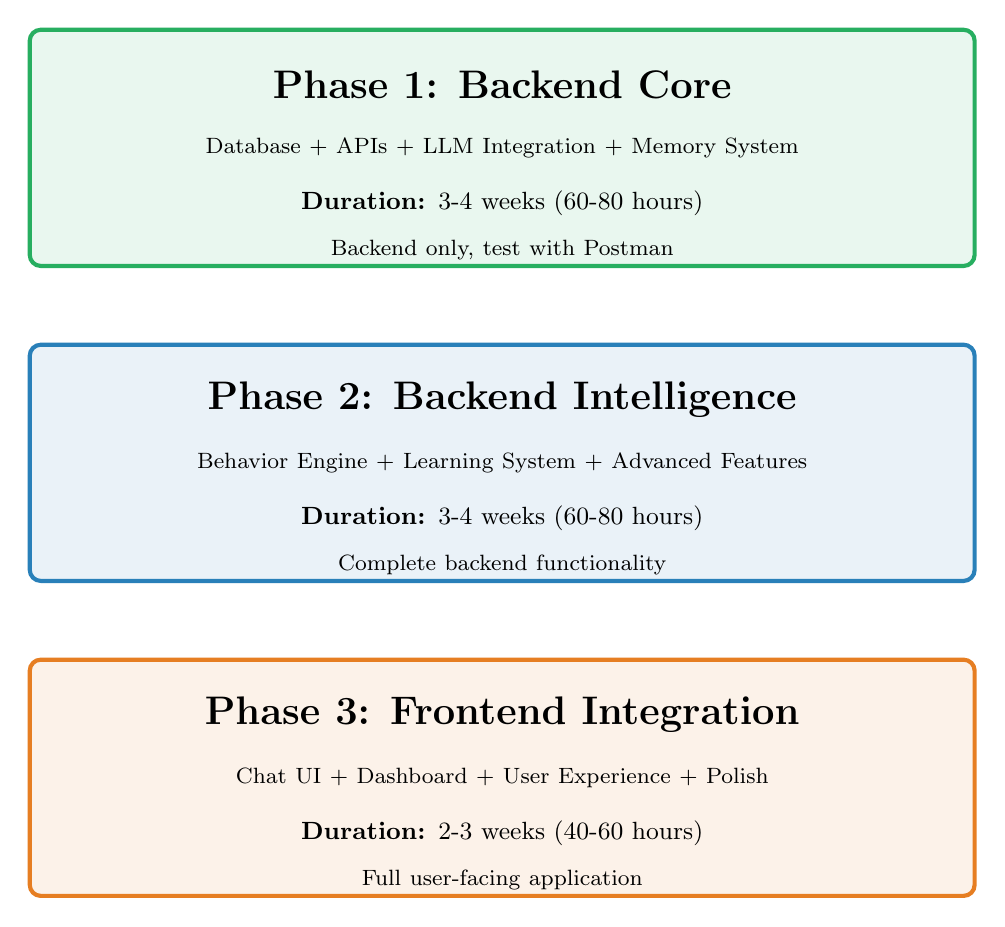
\begin{tikzpicture}[
    node distance=0.3cm,
    every node/.style={font=\small}
]

\foreach \phase/\color/\ypos in {1/switchitgreen/-0, 2/switchitblue/-4, 3/switchitorange/-8} {
    \node[rectangle, rounded corners, minimum width=12cm, minimum height=3cm, draw=\color, line width=1.5pt, fill=\color!10] at (0, \ypos) {};
}

\node at (0, 0.8) {\Large\textbf{Phase 1: Backend Core}};
\node[text width=11cm, align=center] at (0, 0) {\footnotesize Database + APIs + LLM Integration + Memory System};
\node[text width=11cm, align=center] at (0, -0.7) {\small \textbf{Duration:} 3-4 weeks (60-80 hours)};
\node[text width=11cm, align=center] at (0, -1.3) {\footnotesize Backend only, test with Postman};

\node at (0, -3.2) {\Large\textbf{Phase 2: Backend Intelligence}};
\node[text width=11cm, align=center] at (0, -4) {\footnotesize Behavior Engine + Learning System + Advanced Features};
\node[text width=11cm, align=center] at (0, -4.7) {\small \textbf{Duration:} 3-4 weeks (60-80 hours)};
\node[text width=11cm, align=center] at (0, -5.3) {\footnotesize Complete backend functionality};

\node at (0, -7.2) {\Large\textbf{Phase 3: Frontend Integration}};
\node[text width=11cm, align=center] at (0, -8) {\footnotesize Chat UI + Dashboard + User Experience + Polish};
\node[text width=11cm, align=center] at (0, -8.7) {\small \textbf{Duration:} 2-3 weeks (40-60 hours)};
\node[text width=11cm, align=center] at (0, -9.3) {\footnotesize Full user-facing application};

\end{tikzpicture}
\end{center}

\vspace{0.5cm}
\textbf{Total Timeline:} 8-11 weeks (160-220 hours) for complete MVP

\textbf{Working Schedule:} Assuming 20 hours/week → 2-3 months calendar time

\newpage

\subsection{Phase 1: Backend Core (3-4 Weeks)}

\begin{tcolorbox}[colback=switchitgreen!5,colframe=switchitgreen,title=\textbf{Phase 1 Goal}]
Build the complete backend foundation: database, APIs, LLM integration, and basic memory system. \textbf{No frontend yet} — test everything with Postman/Thunder Client.
\end{tcolorbox}

\subsubsection{Week 1: Foundation \& Setup}

\paragraph{Tasks:}
\begin{enumerate}[leftmargin=*]
    \item \textbf{Project Setup}
    \begin{itemize}
        \item Initialize Node.js/NestJS project (or Python/FastAPI)
        \item Set up PostgreSQL database locally
        \item Configure environment variables
        \item Set up Git repository
    \end{itemize}
    
    \item \textbf{Database Design}
    \begin{itemize}
        \item Create `users` table (integrate with existing SwitchIt users)
        \item Create `conversations` table (store all chats)
        \item Create `user\_profiles` table (goals, career stage, emotional state)
        \item Create `memories` table (important events, achievements)
        \item Write migration scripts
    \end{itemize}
    
    \item \textbf{OpenAI API Integration}
    \begin{itemize}
        \item Set up OpenAI API account
        \item Create basic chat completion function
        \item Test with simple prompts
        \item Implement error handling for API failures
    \end{itemize}
\end{enumerate}

\paragraph{Gen AI Helper Prompts:}
\begin{itemize}
    \item "Generate a NestJS project structure for an AI chatbot API"
    \item "Create PostgreSQL schema for storing user conversations with goals and memories"
    \item "Write a TypeScript function to call OpenAI Chat Completion API with error handling"
\end{itemize}

\paragraph{Deliverables:}
\begin{itemize}
    \item Working project structure
    \item Database created and migrated
    \item Basic OpenAI integration tested
\end{itemize}

\subsubsection{Week 2: Core Chat API}

\paragraph{Tasks:}
\begin{enumerate}[leftmargin=*]
    \item \textbf{Chat Endpoint}
    \begin{itemize}
        \item POST /api/companion/chat endpoint
        \item Accept user message, return AI response
        \item Store conversation in database
        \item Retrieve conversation history for context
    \end{itemize}
    
    \item \textbf{System Prompt Engineering}
    \begin{itemize}
        \item Design mentor persona prompt
        \item Include user context (name, profile, goals)
        \item Test different prompt variations
        \item Optimize for helpful, empathetic responses
    \end{itemize}
    
    \item \textbf{Session Management}
    \begin{itemize}
        \item Implement user authentication (JWT tokens)
        \item Track conversation sessions
        \item Load last 10 messages as context
    \end{itemize}
\end{enumerate}

\paragraph{Gen AI Helper Prompts:}
\begin{itemize}
    \item "Create a NestJS controller for a chat API with OpenAI integration"
    \item "Write a system prompt for an AI career mentor that's empathetic and actionable"
    \item "Implement JWT authentication middleware in NestJS"
\end{itemize}

\paragraph{Testing with Postman:}
\begin{itemize}
    \item Send test messages, verify responses
    \item Check database for stored conversations
    \item Test conversation context retrieval
    \item Verify authentication works
\end{itemize}

\subsubsection{Week 3: Memory \& Context}

\paragraph{Tasks:}
\begin{enumerate}[leftmargin=*]
    \item \textbf{User Profile API}
    \begin{itemize}
        \item GET/POST /api/companion/profile
        \item Store user goals, career stage
        \item Update emotional state based on conversations
    \end{itemize}
    
    \item \textbf{SwitchIt Integration}
    \begin{itemize}
        \item Create service to fetch SwitchIt user data
        \item Get user's recent posts, job applications
        \item Include this context in AI prompts
    \end{itemize}
    
    \item \textbf{Smart Context Builder}
    \begin{itemize}
        \item Function that assembles user context for AI
        \item Includes: profile, recent conversations, goals, SwitchIt activity
        \item Keeps total token count under limit
    \end{itemize}
\end{enumerate}

\paragraph{Gen AI Helper Prompts:}
\begin{itemize}
    \item "Create a service to build AI context from user profile, goals, and conversation history"
    \item "Write a function to summarize long conversation history to fit token limits"
\end{itemize}

\subsubsection{Week 4: Goals \& Events Tracking}

\paragraph{Tasks:}
\begin{enumerate}[leftmargin=*]
    \item \textbf{Goals Management}
    \begin{itemize}
        \item GET/POST/PATCH /api/companion/goals endpoints
        \item Create, update, complete goals
        \item Track goal progress
    \end{itemize}
    
    \item \textbf{Event Logging}
    \begin{itemize}
        \item POST /api/companion/events endpoint
        \item Log significant events (interview, job offer, rejection)
        \item Store emotional impact
        \item Reference events in future conversations
    \end{itemize}
    
    \item \textbf{Testing \& Documentation}
    \begin{itemize}
        \item Comprehensive Postman tests for all endpoints
        \item Write API documentation
        \item Add code comments
        \item Fix bugs discovered during testing
    \end{itemize}
\end{enumerate}

\paragraph{Success Criteria:}
\begin{itemize}
    \item All API endpoints work correctly
    \item AI provides contextual responses based on user history
    \item Goals can be created and tracked
    \item Events properly logged
    \item Full Postman collection tests pass
\end{itemize}

\paragraph{Hours Breakdown:}
\begin{itemize}
    \item Week 1: 15-20 hours (setup, database, OpenAI)
    \item Week 2: 15-20 hours (chat API, prompts, auth)
    \item Week 3: 15-20 hours (memory, context, integration)
    \item Week 4: 15-20 hours (goals, events, testing)
    \item \textbf{Total:} 60-80 hours
\end{itemize}

\newpage

\subsection{Phase 2: Persistent Memory (1-2 Months)}

\begin{tcolorbox}[colback=switchitblue!5,colframe=switchitblue,title=\textbf{Phase 2 Goal}]
Transform the companion from a session-based chatbot into a persistent mentor that remembers the user's entire history and responds with emotional intelligence.
\end{tcolorbox}

\subsubsection{What Gets Built}

\begin{itemize}[leftmargin=*]
    \item \textbf{Long-Term Memory:} Store all conversations, goals, and events permanently
    \item \textbf{Vector Database:} Enable semantic search (find relevant past conversations)
    \item \textbf{User Profile System:} Track goals, career stage, emotional state
    \item \textbf{SwitchIt Integration:} Pull data from user's profile, posts, applications
    \item \textbf{Behavior Engine:} AI adapts responses based on user's emotional state
    \item \textbf{Memory Dashboard:} Users can view their tracked goals and progress
\end{itemize}

\subsubsection{Success Criteria}

\begin{itemize}
    \item AI recalls conversations from weeks/months ago
    \item Responses feel personalized and context-aware
    \item Users can set and track goals within the companion
    \item AI detects emotional tone with 70\%+ accuracy
    \item \textbf{Target:} 500+ active users, 60\% return within 7 days
\end{itemize}

\subsubsection{Resources Needed}

\begin{table}[h]
\centering
\begin{tabular}{|l|l|}
\hline
\textbf{Role} & \textbf{Effort} \\
\hline
Backend Developer & 120-160 hours \\
\hline
AI/ML Engineer & 80-100 hours \\
\hline
Frontend Developer & 60-80 hours \\
\hline
Data Engineer & 40-60 hours \\
\hline
Product Manager & 40 hours \\
\hline
\textbf{Total Team Time} & \textbf{340-440 hours} \\
\hline
\end{tabular}
\end{table}

\subsubsection{Key Deliverables}

\begin{enumerate}
    \item Vector database integrated (Pinecone/Qdrant)
    \item Extended database schema with goals, events, user profiles
    \item Memory retrieval system that contextualizes responses
    \item Behavior engine with emotional state detection
    \item Dashboard UI for viewing goals and progress
    \item Privacy controls (delete memory, export data)
\end{enumerate}

\subsubsection{Risks \& Mitigation}

\begin{table}[h]
\centering
\begin{tabularx}{\textwidth}{|l|X|X|}
\hline
\textbf{Risk} & \textbf{Impact} & \textbf{Mitigation} \\
\hline
Privacy concerns & User distrust & Clear privacy policy, user controls \\
\hline
Complex architecture & Development delays & Incremental rollout, strong testing \\
\hline
Vector DB costs & Budget overrun & Start with free tier, monitor usage \\
\hline
\end{tabularx}
\end{table}

\newpage

\subsection{Phase 3: Learning Engine (2-3 Months)}

\begin{tcolorbox}[colback=switchitorange!5,colframe=switchitorange,title=\textbf{Phase 3 Goal}]
Transform the companion from a conversational mentor into an active learning platform with quizzes, challenges, and personalized skill development.
\end{tcolorbox}

\subsubsection{What Gets Built}

\begin{itemize}[leftmargin=*]
    \item \textbf{Quiz Generator:} AI creates custom quizzes based on user's goals
    \item \textbf{Skill Gap Detection:} Identifies weaknesses from conversations and quiz results
    \item \textbf{Learning Roadmaps:} Generates structured learning paths (e.g., "5-day system design plan")
    \item \textbf{Micro-Learning Tasks:} Daily/weekly bite-sized challenges
    \item \textbf{Spaced Repetition:} Revisits topics at optimal intervals for retention
    \item \textbf{Gamification:} Badges, streaks, and progress rewards
\end{itemize}

\subsubsection{Success Criteria}

\begin{itemize}
    \item 60\% of users complete at least one quiz
    \item Average learning plan completion rate: 50\%+
    \item Users report improved interview/job performance
    \item Daily engagement increases by 30\%
    \item \textbf{Target:} 2,000+ active users, 40\% daily active rate
\end{itemize}

\subsubsection{Resources Needed}

\begin{table}[h]
\centering
\begin{tabular}{|l|l|}
\hline
\textbf{Role} & \textbf{Effort} \\
\hline
AI/ML Engineer & 100-120 hours \\
\hline
Backend Developer & 80-100 hours \\
\hline
Frontend Developer & 80-100 hours \\
\hline
Content Specialist & 60-80 hours \\
\hline
UI/UX Designer & 40-60 hours \\
\hline
Product Manager & 40 hours \\
\hline
\textbf{Total Team Time} & \textbf{400-500 hours} \\
\hline
\end{tabular}
\end{table}

\subsubsection{Key Deliverables}

\begin{enumerate}
    \item Quiz generation system with multiple question types
    \item Skill assessment algorithm
    \item Learning roadmap UI with progress tracking
    \item Daily challenge system with notifications
    \item Gamification elements (badges, leaderboards)
    \item Analytics dashboard for user learning metrics
\end{enumerate}

\subsubsection{Risks \& Mitigation}

\begin{table}[h]
\centering
\begin{tabularx}{\textwidth}{|l|X|X|}
\hline
\textbf{Risk} & \textbf{Impact} & \textbf{Mitigation} \\
\hline
Poor content quality & Users disengage & Human review of AI-generated content \\
\hline
Overwhelming users & Decreased usage & Start with optional features, gradual rollout \\
\hline
Low completion rates & Feature underused & A/B test incentives, improve UX \\
\hline
\end{tabularx}
\end{table}

\newpage

\subsection{Phase 4: Intelligent Mentor (3-6 Months)}

\begin{tcolorbox}[colback=switchitpurple!5,colframe=switchitpurple,title=\textbf{Phase 4 Goal}]
Evolve the companion into a proactive, predictive mentor that anticipates user needs and provides strategic career guidance using advanced AI.
\end{tcolorbox}

\subsubsection{What Gets Built}

\begin{itemize}[leftmargin=*]
    \item \textbf{Proactive Interventions:} AI reaches out when it detects user needs help
    \item \textbf{Pattern Recognition:} ML models detect long-term behavioral patterns
    \item \textbf{Career Trajectory Modeling:} Predict likely career paths and suggest optimizations
    \item \textbf{Advanced Personalization:} Multiple response modes (mentor, coach, analyst)
    \item \textbf{Predictive Nudging:} Suggest actions before user asks
    \item \textbf{Journey Timeline:} Visual representation of user's growth over time
    \item \textbf{A/B Testing Engine:} Optimize response strategies based on outcomes
\end{itemize}

\subsubsection{Success Criteria}

\begin{itemize}
    \item 70\%+ user retention over 60 days
    \item Users report 30\% improvement in career confidence
    \item 50\%+ of users achieve at least one major goal
    \item AI proactive messages have 60\%+ engagement rate
    \item \textbf{Target:} 10,000+ active users, 50\% weekly active rate
\end{itemize}

\subsubsection{Resources Needed}

\begin{table}[h]
\centering
\begin{tabular}{|l|l|}
\hline
\textbf{Role} & \textbf{Effort} \\
\hline
Senior ML Engineer & 150-200 hours \\
\hline
Backend Developer & 100-120 hours \\
\hline
Frontend Developer & 80-100 hours \\
\hline
Data Scientist & 80-100 hours \\
\hline
UI/UX Designer & 60-80 hours \\
\hline
Product Manager & 60 hours \\
\hline
\textbf{Total Team Time} & \textbf{530-660 hours} \\
\hline
\end{tabular}
\end{table}

\subsubsection{Key Deliverables}

\begin{enumerate}
    \item ML-based behavior prediction model
    \item Proactive notification system
    \item Multiple AI personalities/modes
    \item Career trajectory visualization
    \item Journey timeline UI
    \item Advanced analytics and insights dashboard
    \item A/B testing infrastructure
\end{enumerate}

\subsubsection{Risks \& Mitigation}

\begin{table}[h]
\centering
\begin{tabularx}{\textwidth}{|l|X|X|}
\hline
\textbf{Risk} & \textbf{Impact} & \textbf{Mitigation} \\
\hline
Creepy factor (too proactive) & User discomfort & User controls, opt-in features \\
\hline
ML model inaccuracy & Poor predictions & Extensive training data, validation \\
\hline
High infrastructure costs & Budget issues & Cost optimization, cloud efficiency \\
\hline
Complexity creep & Maintenance burden & Strong documentation, modular design \\
\hline
\end{tabularx}
\end{table}

%===========================================
\section{Integration with Existing SwitchIt Platform}
%===========================================

\subsection{Integration Points}

The Companion AI connects to SwitchIt in four key areas:

\begin{center}
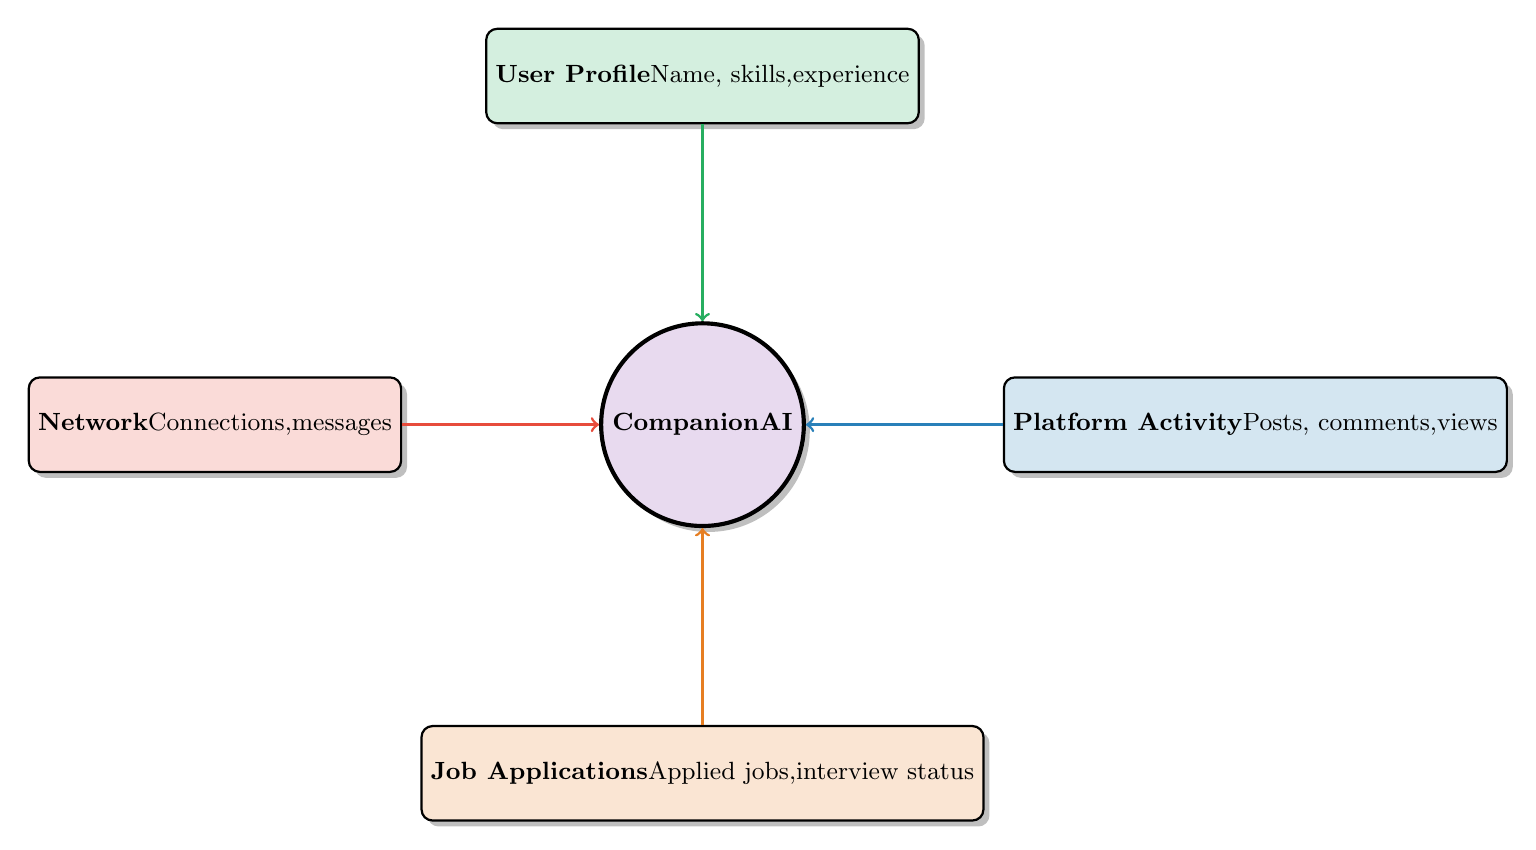
\begin{tikzpicture}[
    node distance=3cm,
    every node/.style={font=\small},
    central/.style={circle, minimum size=2.5cm, text centered, draw=black, line width=1.5pt, fill=switchitpurple!20, drop shadow},
    integration/.style={rectangle, rounded corners, minimum width=2.5cm, minimum height=1.2cm, text centered, draw=black, line width=0.8pt, drop shadow}
]

\node[central] (companion) {\textbf{Companion\\AI}};

\node[integration, fill=switchitgreen!20, above=2.5cm of companion] (profile) {\textbf{User Profile}\\Name, skills,\\experience};

\node[integration, fill=switchitblue!20, right=2.5cm of companion] (activity) {\textbf{Platform Activity}\\Posts, comments,\\views};

\node[integration, fill=switchitorange!20, below=2.5cm of companion] (jobs) {\textbf{Job Applications}\\Applied jobs,\\interview status};

\node[integration, fill=switchitred!20, left=2.5cm of companion] (network) {\textbf{Network}\\Connections,\\messages};

\draw[->, line width=1pt, switchitgreen] (profile) -- (companion);
\draw[->, line width=1pt, switchitblue] (activity) -- (companion);
\draw[->, line width=1pt, switchitorange] (jobs) -- (companion);
\draw[->, line width=1pt, switchitred] (network) -- (companion);

\end{tikzpicture}
\end{center}

\subsection{Data Access Requirements}

\begin{table}[h]
\centering
\begin{tabularx}{\textwidth}{|l|X|l|}
\hline
\textbf{SwitchIt Data} & \textbf{How Companion Uses It} & \textbf{Phase} \\
\hline
User Profile & Personalize responses with user's background & Phase 1 \\
\hline
Career Goals & Track progress, provide relevant guidance & Phase 2 \\
\hline
Posts \& Activity & Understand interests, engagement patterns & Phase 2 \\
\hline
Job Applications & Offer interview prep, celebrate successes & Phase 2 \\
\hline
Skill Endorsements & Identify strengths, suggest development areas & Phase 3 \\
\hline
Network Activity & Suggest networking strategies & Phase 4 \\
\hline
Search History & Predict career interests & Phase 4 \\
\hline
\end{tabularx}
\caption{SwitchIt Platform Data Integration}
\end{table}

\subsection{Backend API Integration}

\paragraph{What Needs to Happen:}

\begin{enumerate}[leftmargin=*]
    \item \textbf{Create API Endpoints:} SwitchIt backend exposes user data to Companion service
    \item \textbf{Authentication:} Secure connection between platforms (OAuth/JWT tokens)
    \item \textbf{Real-Time Updates:} When user updates profile/applies to job, Companion is notified
    \item \textbf{Event Webhooks:} SwitchIt sends events (job application, post published) to Companion
    \item \textbf{Database Access:} Companion reads from SwitchIt database (read-only for security)
\end{enumerate}

\paragraph{Security Considerations:}

\begin{itemize}
    \item All data transfer encrypted (HTTPS/TLS)
    \item Companion only accesses data for authenticated user
    \item No third-party data sharing
    \item Audit logs for data access
    \item User consent required for data usage
\end{itemize}

%===========================================
\section{Success Metrics \& KPIs}
%===========================================

\subsection{User Engagement Metrics}

\begin{table}[h]
\centering
\begin{tabularx}{\textwidth}{|l|X|l|l|}
\hline
\textbf{Metric} & \textbf{Definition} & \textbf{Target} & \textbf{Phase} \\
\hline
Daily Active Users (DAU) & Users chatting daily & 40\% of total & P3-P4 \\
\hline
Weekly Active Users (WAU) & Users active weekly & 60\% of total & P2+ \\
\hline
Session Duration & Time per chat session & 5+ minutes & P1+ \\
\hline
Messages per Session & Average messages exchanged & 8-10 & P1+ \\
\hline
Return Rate (7-day) & Users return within 7 days & 60\% & P2+ \\
\hline
Return Rate (30-day) & Users return within 30 days & 70\% & P3-P4 \\
\hline
\end{tabularx}
\caption{Engagement KPIs}
\end{table}

\subsection{Learning \& Growth Metrics}

\begin{table}[h]
\centering
\begin{tabularx}{\textwidth}{|l|X|l|l|}
\hline
\textbf{Metric} & \textbf{Definition} & \textbf{Target} & \textbf{Phase} \\
\hline
Quiz Completion Rate & \% of started quizzes completed & 60\% & P3 \\
\hline
Learning Plan Adherence & \% following daily learning tasks & 50\% & P3 \\
\hline
Goal Achievement Rate & \% of goals marked complete & 40-50\% & P2+ \\
\hline
Skill Improvement & Self-reported skill growth & +30\% & P3-P4 \\
\hline
\end{tabularx}
\caption{Learning KPIs}
\end{table}

\subsection{Business Impact Metrics}

\begin{table}[h]
\centering
\begin{tabularx}{\textwidth}{|l|X|l|}
\hline
\textbf{Metric} & \textbf{Definition} & \textbf{Target} \\
\hline
Platform Retention & Users staying on SwitchIt overall & +25\% \\
\hline
Job Success Rate & Users getting jobs after using Companion & +20\% \\
\hline
User Satisfaction (NPS) & Net Promoter Score for Companion & 50+ \\
\hline
Referral Rate & Users recommending SwitchIt to others & +15\% \\
\hline
Premium Conversion & Free to paid user conversion (if monetized) & 10-15\% \\
\hline
\end{tabularx}
\caption{Business KPIs}
\end{table}

\subsection{Technical Performance Metrics}

\begin{table}[h]
\centering
\begin{tabularx}{\textwidth}{|l|X|l|}
\hline
\textbf{Metric} & \textbf{Definition} & \textbf{Target} \\
\hline
Response Time & Time from user message to AI response & < 3 seconds \\
\hline
Uptime & System availability & 99.5\%+ \\
\hline
Error Rate & Failed requests & < 1\% \\
\hline
Memory Retrieval Accuracy & Relevant context retrieved & 85\%+ \\
\hline
\end{tabularx}
\caption{Technical KPIs}
\end{table}

%===========================================
\section{Resource Planning}
%===========================================

\subsection{Team Composition}

\begin{table}[h]
\centering
\begin{tabularx}{\textwidth}{|l|X|l|}
\hline
\textbf{Role} & \textbf{Responsibilities} & \textbf{FTE} \\
\hline
Product Manager & Strategy, roadmap, user research & 0.5-1.0 \\
\hline
Frontend Developer & Chat UI, dashboard, mobile responsive & 1-2 \\
\hline
Backend Developer & APIs, integration, infrastructure & 1-2 \\
\hline
AI/ML Engineer & LLM integration, behavior engine, models & 1-2 \\
\hline
Data Engineer & Database design, vector DB, analytics & 0.5-1.0 \\
\hline
UI/UX Designer & Interface design, user flows & 0.5 \\
\hline
QA Engineer & Testing, quality assurance & 0.5 \\
\hline
DevOps Engineer & Deployment, monitoring, scaling & 0.5 \\
\hline
\textbf{Total Team} & & \textbf{6-10 FTE} \\
\hline
\end{tabularx}
\caption{Team Resource Requirements}
\end{table}

\subsection{Budget Estimation}

\begin{table}[h]
\centering
\begin{tabularx}{\textwidth}{|l|X|r|}
\hline
\textbf{Category} & \textbf{Description} & \textbf{Est. Cost (Annual)} \\
\hline
Personnel & Team salaries (6-10 people) & \$500K - \$1M \\
\hline
AI API Costs & OpenAI/Claude API usage & \$20K - \$50K \\
\hline
Infrastructure & AWS/GCP servers, databases & \$30K - \$60K \\
\hline
Vector Database & Pinecone/Qdrant subscription & \$5K - \$15K \\
\hline
Tools \& Software & Development tools, licenses & \$10K - \$20K \\
\hline
Contingency & Unexpected costs (15\%) & \$85K - \$172K \\
\hline
\textbf{Total (Year 1)} & & \textbf{\$650K - \$1.3M} \\
\hline
\end{tabularx}
\caption{Budget Breakdown}
\end{table}

\textit{Note: Costs scale with user volume. Estimates assume 10K-50K users by end of Year 1.}

\subsection{Timeline Overview}

\begin{center}
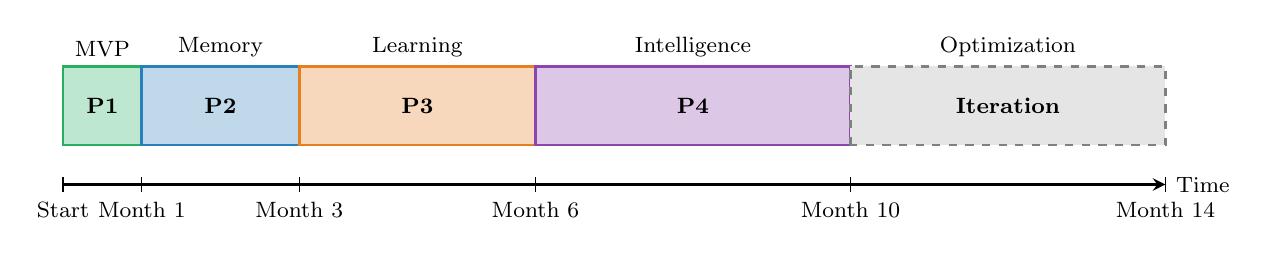
\begin{tikzpicture}[
    every node/.style={font=\footnotesize}
]

% Timeline axis
\draw[line width=1pt, ->, >=stealth] (0,0) -- (14,0) node[right] {Time};

% Phase markers
\foreach \x/\label in {0/Start, 1/Month 1, 3/Month 3, 6/Month 6, 10/Month 10, 14/Month 14} {
    \draw (\x, -0.1) -- (\x, 0.1);
    \node[below] at (\x, -0.1) {\label};
}

% Phase 1
\draw[fill=switchitgreen!30, draw=switchitgreen, line width=1pt] (0, 0.5) rectangle (1, 1.5);
\node at (0.5, 1) {\textbf{P1}};
\node[above] at (0.5, 1.5) {MVP};

% Phase 2
\draw[fill=switchitblue!30, draw=switchitblue, line width=1pt] (1, 0.5) rectangle (3, 1.5);
\node at (2, 1) {\textbf{P2}};
\node[above] at (2, 1.5) {Memory};

% Phase 3
\draw[fill=switchitorange!30, draw=switchitorange, line width=1pt] (3, 0.5) rectangle (6, 1.5);
\node at (4.5, 1) {\textbf{P3}};
\node[above] at (4.5, 1.5) {Learning};

% Phase 4
\draw[fill=switchitpurple!30, draw=switchitpurple, line width=1pt] (6, 0.5) rectangle (10, 1.5);
\node at (8, 1) {\textbf{P4}};
\node[above] at (8, 1.5) {Intelligence};

% Post-launch
\draw[fill=gray!20, draw=gray, line width=1pt, dashed] (10, 0.5) rectangle (14, 1.5);
\node at (12, 1) {\textbf{Iteration}};
\node[above] at (12, 1.5) {Optimization};

\end{tikzpicture}
\end{center}

\textbf{Total Development Time:} 10-14 months from start to full launch

%===========================================
\section{Risks \& Mitigation Strategies}
%===========================================

\subsection{Critical Risks}

\begin{table}[h]
\centering
\begin{tabularx}{\textwidth}{|l|l|X|X|}
\hline
\textbf{Risk} & \textbf{Probability} & \textbf{Impact} & \textbf{Mitigation Strategy} \\
\hline
Poor AI response quality & Medium & High & Extensive prompt engineering, GPT-4, human oversight \\
\hline
Privacy/security breach & Low & Critical & Encryption, audit logs, compliance review, penetration testing \\
\hline
Low user adoption & Medium & High & Beta testing, user feedback loops, marketing campaign \\
\hline
High infrastructure costs & Medium & Medium & Cost monitoring, cloud optimization, tiered rollout \\
\hline
Integration complexity & Medium & Medium & Modular architecture, incremental integration, testing \\
\hline
Competitive features & Low & Medium & Fast iteration, unique value prop, user loyalty \\
\hline
Regulatory issues (AI/data) & Low & High & Legal review, GDPR compliance, transparency \\
\hline
\end{tabularx}
\caption{Risk Assessment Matrix}
\end{table}

\subsection{Contingency Plans}

\paragraph{If User Adoption is Low (<100 active users in Phase 1):}
\begin{itemize}
    \item Conduct user interviews to identify friction points
    \item Improve onboarding flow and initial experience
    \item Add incentives (gamification, exclusive features)
    \item Adjust marketing messaging
\end{itemize}

\paragraph{If Infrastructure Costs Exceed Budget:}
\begin{itemize}
    \item Switch to lower-cost AI models for non-critical interactions
    \item Implement aggressive caching strategies
    \item Negotiate volume discounts with providers
    \item Consider building some components in-house
\end{itemize}

\paragraph{If Development Timeline Slips:}
\begin{itemize}
    \item Reduce scope of current phase, move features to next phase
    \item Add temporary contractor support
    \item Parallelize independent workstreams
    \item Extend beta period, delay public launch
\end{itemize}

%===========================================
\section{Privacy, Security \& Ethics}
%===========================================

\subsection{Privacy Principles}

\begin{enumerate}[leftmargin=*]
    \item \textbf{Transparency:} Users know exactly what data is stored and why
    \item \textbf{Consent:} Explicit opt-in for memory storage with clear explanation
    \item \textbf{Control:} Users can view, export, or delete all their data anytime
    \item \textbf{Minimization:} Only collect data necessary for functionality
    \item \textbf{Protection:} Encryption at rest and in transit
    \item \textbf{No Third-Party Sharing:} User data never sold or shared without consent
\end{enumerate}

\subsection{User-Facing Privacy Controls}

\begin{itemize}
    \item \textbf{Memory Toggle:} Turn off long-term memory (session-only mode)
    \item \textbf{Selective Deletion:} Delete specific conversations or memories
    \item \textbf{Complete Reset:} Wipe all Companion data and start fresh
    \item \textbf{Data Export:} Download all conversations and profile data
    \item \textbf{View What AI Knows:} See full profile and memory contents
    \item \textbf{Pause Learning:} Stop AI from tracking progress temporarily
\end{itemize}

\subsection{Ethical AI Guidelines}

\begin{enumerate}[leftmargin=*]
    \item \textbf{No Manipulation:} AI encourages growth but never manipulates emotions
    \item \textbf{No Judgment:} Supportive tone, never critical or condescending
    \item \textbf{Human Boundaries:} AI clarifies it's not a replacement for human relationships
    \item \textbf{Honest Limitations:} AI acknowledges when it doesn't know something
    \item \textbf{Bias Mitigation:} Regular audits for gender, racial, or cultural bias
    \item \textbf{Mental Health Safeguards:} Recognize crisis language, suggest professional help
\end{enumerate}

\subsection{Compliance Requirements}

\begin{itemize}
    \item \textbf{GDPR:} Right to access, portability, erasure (EU users)
    \item \textbf{CCPA:} California privacy rights compliance
    \item \textbf{SOC 2:} Security and availability standards
    \item \textbf{Terms of Service:} Clear legal agreement for Companion usage
    \item \textbf{Privacy Policy:} Detailed data handling documentation
\end{itemize}

%===========================================
\section{Go-to-Market Strategy}
%===========================================

\subsection{Launch Approach}

\begin{enumerate}[leftmargin=*]
    \item \textbf{Private Beta (Phase 1):}
    \begin{itemize}
        \item Invite 100-200 engaged SwitchIt users
        \item Collect intensive feedback
        \item Iterate rapidly based on learnings
        \item Duration: 2-4 weeks
    \end{itemize}
    
    \item \textbf{Limited Public Beta (Phase 2):}
    \begin{itemize}
        \item Open to 1,000 waitlist users
        \item Gradual onboarding (100/week)
        \item A/B test different onboarding flows
        \item Duration: 6-8 weeks
    \end{itemize}
    
    \item \textbf{Soft Launch (Phase 3):}
    \begin{itemize}
        \item Available to all SwitchIt users, opt-in
        \item Marketing push to existing user base
        \item Press release, blog posts
        \item Duration: 2-3 months
    \end{itemize}
    
    \item \textbf{Full Launch (Phase 4):}
    \begin{itemize}
        \item Default feature for all new users
        \item Major marketing campaign
        \item Influencer partnerships
        \item Case studies and testimonials
    \end{itemize}
\end{enumerate}

\subsection{Marketing Messaging}

\paragraph{Primary Value Proposition:}
\begin{center}
\fcolorbox{switchitpurple}{switchitpurple!5}{%
\parbox{0.85\textwidth}{%
\centering
\Large
\textit{"Your Personal AI Mentor Who Remembers Everything and Helps You Grow Every Day"}
}
}
\end{center}

\paragraph{Key Messaging Pillars:}
\begin{enumerate}
    \item \textbf{Never Repeat Yourself:} Unlike therapists or coaches, your AI companion remembers your entire journey
    \item \textbf{Always Available:} 24/7 guidance whenever you need encouragement or advice
    \item \textbf{Truly Personal:} Not generic advice—recommendations based on YOUR goals, history, and style
    \item \textbf{Action-Oriented:} Not just talk—get quizzes, challenges, and concrete next steps
    \item \textbf{Growth Tracking:} See your progress over weeks and months with clear visualizations
\end{enumerate}

\subsection{Target User Segments (Priority Order)}

\begin{enumerate}
    \item \textbf{Active Job Seekers:} Users applying to jobs, need interview prep and motivation
    \item \textbf{Career Switchers:} Professionals changing industries, need skill development
    \item \textbf{Early Career:} Recent grads figuring out their path, need guidance
    \item \textbf{High Achievers:} Ambitious professionals seeking continuous growth
    \item \textbf{Returnees:} People returning to workforce after break, need confidence
\end{enumerate}

%===========================================
\section{Future Vision \& Expansion}
%===========================================

\subsection{Potential Enhancements (Beyond Phase 4)}

\begin{enumerate}[leftmargin=*]
    \item \textbf{Voice Interface:} Talk to your companion via voice commands
    \item \textbf{Mobile App:} Native iOS/Android companion app for on-the-go
    \item \textbf{Multi-language Support:} Expand to non-English speaking markets
    \item \textbf{Expert Matching:} AI connects you with human mentors based on your needs
    \item \textbf{Group Challenges:} Collaborate with other SwitchIt users on learning goals
    \item \textbf{Resume Optimization:} AI analyzes and improves your SwitchIt profile/resume
    \item \textbf{Interview Simulator:} Practice interviews with AI in realistic scenarios
    \item \textbf{Career Path Visualization:} Interactive tree showing possible career trajectories
    \item \textbf{Calendar Integration:} Schedule learning sessions and reminders
    \item \textbf{Anonymous Benchmarking:} Compare your progress with similar professionals
\end{enumerate}

\subsection{Monetization Opportunities}

\begin{table}[h]
\centering
\begin{tabularx}{\textwidth}{|l|X|l|}
\hline
\textbf{Model} & \textbf{Description} & \textbf{Potential} \\
\hline
Freemium & Basic free, premium features paid & High \\
\hline
Subscription & Monthly/annual for full access & Medium \\
\hline
Enterprise & B2B for companies training employees & High \\
\hline
Certifications & Paid certificates for completed learning paths & Medium \\
\hline
Premium Content & Expert-created courses and resources & Medium \\
\hline
\end{tabularx}
\caption{Monetization Options}
\end{table}

\subsection{Long-Term Vision}

\begin{tcolorbox}[colback=switchitpurple!5,colframe=switchitpurple,title=\textbf{5-Year Vision}]
By 2031, the SwitchIt Companion AI becomes the \textbf{world's most trusted career mentor}, guiding millions of professionals through their career journeys. 

\vspace{0.3cm}

It's not just a feature—it's THE reason people choose SwitchIt over LinkedIn.

\vspace{0.3cm}

Every user has a persistent AI companion that has been with them through job searches, promotions, setbacks, and triumphs—making SwitchIt indispensable for career growth.
\end{tcolorbox}

%===========================================
\section{Backend-Frontend Integration: Technical Deep Dive}
%===========================================

\subsection{Architecture Overview}

The SwitchIt Companion AI follows a modern three-tier architecture with clear separation between presentation (Frontend), business logic (Backend), and data persistence (Database + Vector Store).

\begin{center}
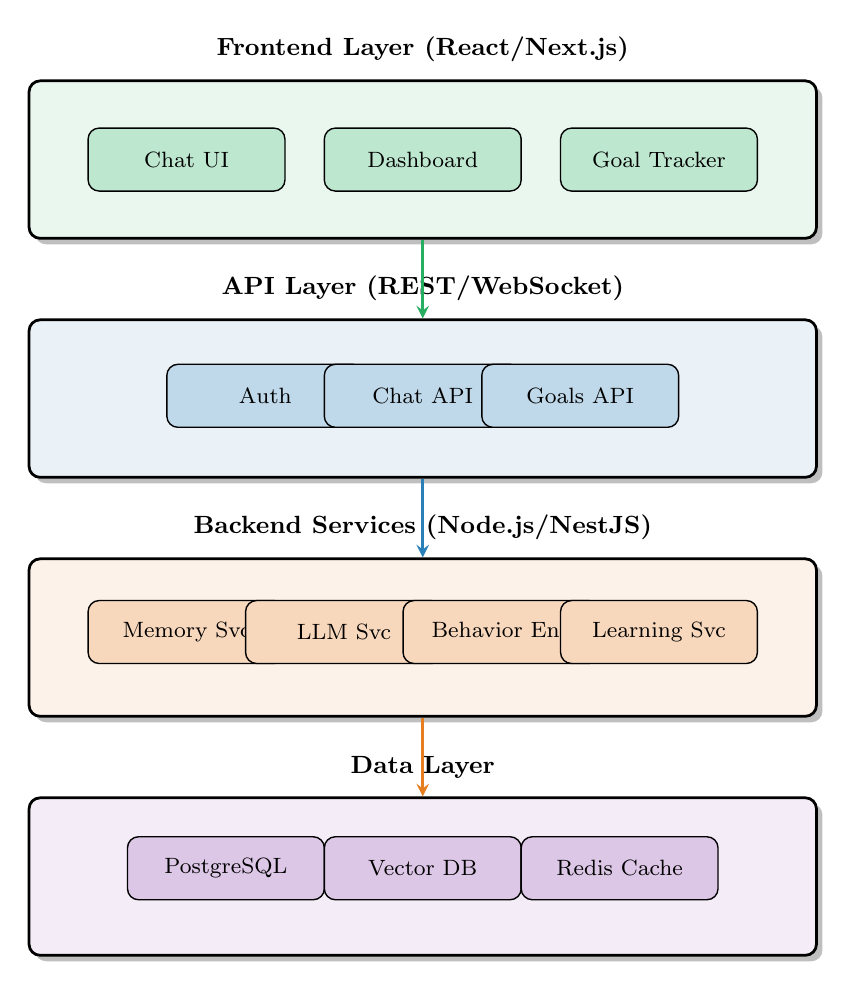
\begin{tikzpicture}[
    node distance=2cm,
    every node/.style={font=\small},
    layer/.style={rectangle, rounded corners, minimum width=10cm, minimum height=2cm, text centered, draw=black, line width=1pt, drop shadow},
    component/.style={rectangle, rounded corners, minimum width=2.5cm, minimum height=0.8cm, text centered, draw=black, line width=0.5pt, font=\footnotesize},
    arrow/.style={->, >=stealth, line width=1pt}
]

% Frontend Layer
\node[layer, fill=switchitgreen!10] (frontend) at (0,0) {};
\node[above=0.1cm of frontend] {\textbf{Frontend Layer (React/Next.js)}};
\node[component, fill=switchitgreen!30] at (-3, 0) {Chat UI};
\node[component, fill=switchitgreen!30] at (0, 0) {Dashboard};
\node[component, fill=switchitgreen!30] at (3, 0) {Goal Tracker};

% API Layer
\node[layer, fill=switchitblue!10, below=1cm of frontend] (api) {};
\node[above=0.1cm of api] {\textbf{API Layer (REST/WebSocket)}};
\node[component, fill=switchitblue!30] at (-2, -3) {Auth};
\node[component, fill=switchitblue!30] at (0, -3) {Chat API};
\node[component, fill=switchitblue!30] at (2, -3) {Goals API};

% Backend Services
\node[layer, fill=switchitorange!10, below=1cm of api] (backend) {};
\node[above=0.1cm of backend] {\textbf{Backend Services (Node.js/NestJS)}};
\node[component, fill=switchitorange!30] at (-3, -6) {Memory Svc};
\node[component, fill=switchitorange!30] at (-1, -6) {LLM Svc};
\node[component, fill=switchitorange!30] at (1, -6) {Behavior Eng};
\node[component, fill=switchitorange!30] at (3, -6) {Learning Svc};

% Data Layer
\node[layer, fill=switchitpurple!10, below=1cm of backend] (data) {};
\node[above=0.1cm of data] {\textbf{Data Layer}};
\node[component, fill=switchitpurple!30] at (-2.5, -9) {PostgreSQL};
\node[component, fill=switchitpurple!30] at (0, -9) {Vector DB};
\node[component, fill=switchitpurple!30] at (2.5, -9) {Redis Cache};

% Arrows
\draw[arrow, switchitgreen] (frontend) -- (api);
\draw[arrow, switchitblue] (api) -- (backend);
\draw[arrow, switchitorange] (backend) -- (data);

\end{tikzpicture}
\end{center}

\subsection{Backend Architecture}

\subsubsection{Service Layer Design}

The backend follows a microservices-inspired modular architecture where each service has a single, well-defined responsibility.

\paragraph{1. Memory Service (\texttt{memory.service.ts})}

\textbf{Purpose:} Manage all conversation storage, retrieval, and context building.

\textbf{Key Functions:}
\begin{itemize}
    \item \texttt{storeMessage(userId, message, sender)}: Save conversation message
    \item \texttt{getConversationHistory(userId, limit)}: Retrieve recent messages
    \item \texttt{semanticSearch(userId, query)}: Find relevant past conversations
    \item \texttt{buildContext(userId)}: Assemble complete user context for AI
\end{itemize}

\textbf{Database Interactions:}
\begin{verbatim}
// Store conversation
INSERT INTO companion_conversations 
  (user_id, message, sender, timestamp, tokens_used)
VALUES ($1, $2, $3, NOW(), $4);

// Semantic search using vector database
SELECT * FROM companion_memories 
WHERE user_id = $1 
ORDER BY embedding_vector <=> $2 
LIMIT 10;
\end{verbatim}

\paragraph{2. LLM Service (\texttt{llm.service.ts})}

\textbf{Purpose:} Interface with OpenAI/Claude APIs for response generation.

\textbf{Key Functions:}
\begin{itemize}
    \item \texttt{generateResponse(context, userMessage)}: Get AI response
    \item \texttt{generateEmbedding(text)}: Create vector embedding
    \item \texttt{estimateTokens(text)}: Calculate token usage
    \item \texttt{streamResponse(context, userMessage)}: Stream AI responses
\end{itemize}

\textbf{OpenAI Integration:}
\begin{verbatim}
const response = await openai.chat.completions.create({
  model: "gpt-4-turbo",
  messages: [
    { role: "system", content: systemPrompt },
    { role: "user", content: userContext },
    { role: "user", content: currentMessage }
  ],
  temperature: 0.7,
  max_tokens: 4096
});
\end{verbatim}

\paragraph{3. Behavior Engine (\texttt{behavior.engine.ts})}

\textbf{Purpose:} Determine AI response strategy based on user state.

\textbf{Decision Logic:}
\begin{verbatim}
function selectResponseMode(userProfile) {
  if (userProfile.emotional_state === 'low') {
    return 'EMPATHY_MODE';
  } else if (userProfile.motivation_level === 'high') {
    return 'CHALLENGE_MODE';
  } else if (userProfile.recent_failure) {
    return 'SUPPORT_MODE';
  } else {
    return 'MENTOR_MODE';
  }
}
\end{verbatim}

\paragraph{4. Learning Service (\texttt{learning.service.ts})}

\textbf{Purpose:} Generate quizzes, learning paths, and track progress.

\textbf{Key Functions:}
\begin{itemize}
    \item \texttt{generateQuiz(userId, topic, difficulty)}: Create quiz
    \item \texttt{evaluateQuizResults(quizId, answers)}: Score and analyze
    \item \texttt{createLearningRoadmap(userId, goal)}: Generate learning plan
    \item \texttt{detectSkillGaps(userId)}: Identify weaknesses
\end{itemize}

\subsubsection{Database Schema Design}

\textbf{Entity Relationship Diagram:}

\begin{center}
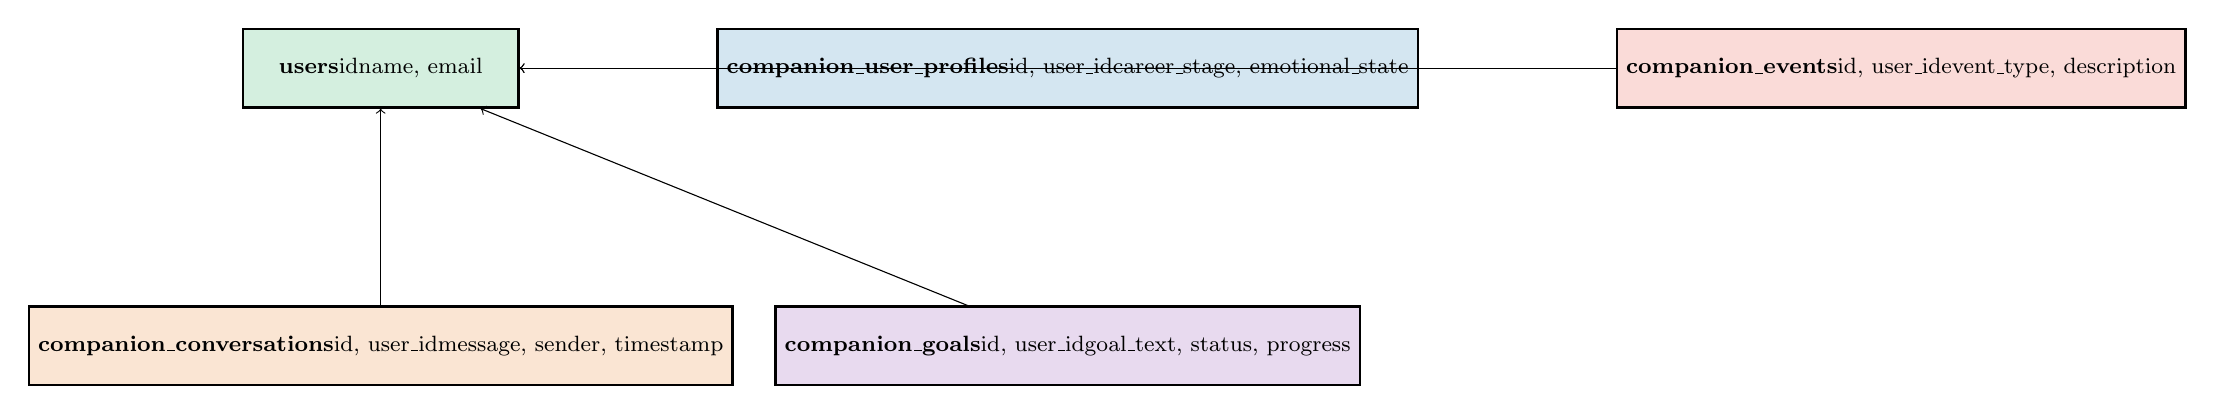
\begin{tikzpicture}[
    node distance=2.5cm,
    every node/.style={font=\footnotesize},
    table/.style={rectangle, draw=black, line width=0.8pt, minimum width=3.5cm, minimum height=1cm},
    pk/.style={font=\tiny\ttfamily, color=switchitblue},
    fk/.style={font=\tiny\ttfamily, color=switchitred}
]

% Tables
\node[table, fill=switchitgreen!20] (users) {
    \textbf{users}\\
    \pk{id}\\
    name, email
};

\node[table, fill=switchitblue!20, right=of users] (profile) {
    \textbf{companion\_user\_profiles}\\
    \pk{id}, \fk{user\_id}\\
    career\_stage, emotional\_state
};

\node[table, fill=switchitorange!20, below=of users] (conv) {
    \textbf{companion\_conversations}\\
    \pk{id}, \fk{user\_id}\\
    message, sender, timestamp
};

\node[table, fill=switchitpurple!20, below=of profile] (goals) {
    \textbf{companion\_goals}\\
    \pk{id}, \fk{user\_id}\\
    goal\_text, status, progress
};

\node[table, fill=switchitred!20, right=of profile] (events) {
    \textbf{companion\_events}\\
    \pk{id}, \fk{user\_id}\\
    event\_type, description
};

% Relationships
\draw[->] (profile) -- (users);
\draw[->] (conv) -- (users);
\draw[->] (goals) -- (users);
\draw[->] (events) -- (users);

\end{tikzpicture}
\end{center}

\newpage

\subsubsection{API Endpoint Specifications}

\textbf{Chat Endpoint - POST /api/v1/companion/chat}

\textit{Purpose:} Send a message to the AI companion and receive a response.

\textbf{Request Body:}
\begin{verbatim}
{
  "message": "I have an interview tomorrow, feeling nervous",
  "session_id": "uuid-session-123"
}
\end{verbatim}

\textbf{Response:}
\begin{verbatim}
{
  "response": "It's completely normal to feel nervous...",
  "metadata": {
    "tokens_used": 256,
    "response_mode": "SUPPORT_MODE",
    "timestamp": "2024-01-24T12:30:00Z"
  }
}
\end{verbatim}

\textbf{Backend Processing Flow:}
\begin{enumerate}
    \item Authenticate user via JWT token
    \item Load user profile and emotional state
    \item Retrieve last 10 conversation messages
    \item Perform semantic search for relevant past conversations
    \item Build complete context (profile + history + SwitchIt data)
    \item Behavior engine selects response mode
    \item Send context to LLM service
    \item Store user message and AI response
    \item Generate embedding for semantic indexing
    \item Return response to frontend
\end{enumerate}

\textbf{Goals Endpoint - POST /api/v1/companion/goals}

\textit{Purpose:} Create a new career goal.

\textbf{Request Body:}
\begin{verbatim}
{
  "goal_text": "Master system design interviews",
  "category": "SKILL_DEVELOPMENT",
  "target_date": "2024-03-01"
}
\end{verbatim}

\textbf{Response:}
\begin{verbatim}
{
  "goal_id": "uuid-goal-456",
  "status": "ACTIVE",
  "progress_percentage": 0,
  "ai_suggestion": "I'll help you achieve this with a 
                    5-day learning plan..."
}
\end{verbatim}

\subsection{Frontend Architecture}

\subsubsection{Component Hierarchy}

\begin{verbatim}
app/
├── layout.tsx                    (Main app layout)
└── dashboard/
    └── page.tsx                  (Dashboard page)

components/
├── CompanionChat/
│   ├── index.tsx                 (Main chat component)
│   ├── MessageList.tsx           (Display messages)
│   ├── MessageInput.tsx          (User input field)
│   ├── TypingIndicator.tsx       (AI typing animation)
│   └── FloatingButton.tsx        (Chat launcher button)
│
├── CompanionDashboard/
│   ├── index.tsx                 (Dashboard layout)
│   ├── GoalsList.tsx             (Display goals)
│   ├── ProgressChart.tsx         (Visualize growth)
│   └── ConversationHistory.tsx   (Past chats)
│
├── GoalTracker/
│   ├── index.tsx                 (Goal management UI)
│   ├── GoalCard.tsx              (Individual goal display)
│   └── CreateGoalModal.tsx       (New goal form)
│
└── LearningHub/
    ├── index.tsx                 (Learning activities)
    ├── QuizCard.tsx              (Quiz display)
    └── RoadmapView.tsx           (Learning path viz)

services/
├── companionAPI.ts               (API client functions)
├── websocket.ts                  (Real-time connection)
└── storage.ts                    (Local state management)
\end{verbatim}

\subsubsection{State Management}

\textbf{Using React Context + Custom Hooks:}

\begin{verbatim}
// CompanionContext.tsx
interface CompanionState {
  messages: Message[];
  userProfile: UserProfile;
  goals: Goal[];
  isTyping: boolean;
}

const CompanionContext = createContext<CompanionState>();

// Custom hook for accessing companion state
export const useCompanion = () => {
  const context = useContext(CompanionContext);
  return context;
};
\end{verbatim}

\textbf{API Client Service:}

\begin{verbatim}
// services/companionAPI.ts
export const companionAPI = {
  async sendMessage(message: string) {
    const response = await fetch('/api/v1/companion/chat', {
      method: 'POST',
      headers: {
        'Content-Type': 'application/json',
        'Authorization': `Bearer ${getAuthToken()}`
      },
      body: JSON.stringify({ message })
    });
    return response.json();
  },
  
  async getGoals() {
    const response = await fetch('/api/v1/companion/goals', {
      headers: { 'Authorization': `Bearer ${getAuthToken()}` }
    });
    return response.json();
  }
};
\end{verbatim}

\subsubsection{Real-Time Communication (WebSockets)}

For streaming AI responses and live updates:

\begin{verbatim}
// Backend WebSocket handler
wss.on('connection', (ws, req) => {
  const userId = authenticateWebSocket(req);
  
  ws.on('message', async (message) => {
    const userMessage = JSON.parse(message);
    
    // Stream AI response word-by-word
    const stream = await llmService.streamResponse(
      userId, 
      userMessage.text
    );
    
    for await (const chunk of stream) {
      ws.send(JSON.stringify({
        type: 'AI_RESPONSE_CHUNK',
        content: chunk
      }));
    }
    
    ws.send(JSON.stringify({ type: 'AI_RESPONSE_COMPLETE' }));
  });
});
\end{verbatim}

\begin{verbatim}
// Frontend WebSocket client
const socket = new WebSocket('wss://api.switchit.com/companion');

socket.onmessage = (event) => {
  const data = JSON.parse(event.data);
  
  if (data.type === 'AI_RESPONSE_CHUNK') {
    appendToCurrentMessage(data.content);
  } else if (data.type === 'AI_RESPONSE_COMPLETE') {
    finalizeMessage();
  }
};
\end{verbatim}

\subsection{Data Flow: Complete User Journey}

\subsubsection{Scenario: User Asks for Career Advice}

\textbf{Step 1: Frontend - User types message}

\begin{verbatim}
// User types in MessageInput component
const handleSendMessage = async () => {
  setMessages([...messages, { 
    sender: 'user', 
    text: inputValue 
  }]);
  setIsTyping(true);
  
  const response = await companionAPI.sendMessage(inputValue);
  
  setMessages(prev => [...prev, { 
    sender: 'ai', 
    text: response.response 
  }]);
  setIsTyping(false);
};
\end{verbatim}

\textbf{Step 2: API Gateway - Authentication \& Routing}

\begin{verbatim}
// Backend middleware
app.post('/api/v1/companion/chat', 
  authenticateJWT,  // Verify user token
  rateLimiter,      // Prevent abuse
  async (req, res) => {
    const { message } = req.body;
    const userId = req.user.id;
    
    const response = await chatController.handleMessage(
      userId, 
      message
    );
    
    res.json(response);
  }
);
\end{verbatim}

\textbf{Step 3: Backend - Context Assembly}

\begin{verbatim}
// chatController.handleMessage()
async function handleMessage(userId, message) {
  // 1. Load user profile
  const profile = await db.query(
    'SELECT * FROM companion_user_profiles WHERE user_id = $1',
    [userId]
  );
  
  // 2. Get conversation history
  const history = await memoryService.getConversationHistory(
    userId, 
    10
  );
  
  // 3. Semantic search for relevant context
  const relevantMemories = await memoryService.semanticSearch(
    userId, 
    message
  );
  
  // 4. Get SwitchIt platform data
  const switchitData = await switchitService.getUserActivity(
    userId
  );
  
  // 5. Build complete context
  const context = contextBuilder.build({
    profile,
    history,
    relevantMemories,
    switchitData,
    currentMessage: message
  });
  
  return context;
}
\end{verbatim}

\textbf{Step 4: Behavior Engine - Determine Response Mode}

\begin{verbatim}
const responseMode = behaviorEngine.selectMode({
  emotional_state: profile.emotional_state,
  recent_events: profile.recent_events,
  motivation_level: profile.motivation_level
});

// Adjust system prompt based on mode
const systemPrompt = getSystemPrompt(responseMode);
// Example: "You are an empathetic career mentor..."
\end{verbatim}

\textbf{Step 5: LLM Service - Generate Response}

\begin{verbatim}
const aiResponse = await llmService.generateResponse({
  systemPrompt,
  context,
  userMessage: message
});

// OpenAI API call happens here
\end{verbatim}

\textbf{Step 6: Memory Service - Store Conversation}

\begin{verbatim}
// Store user message
await db.query(
  'INSERT INTO companion_conversations 
   (user_id, message, sender, timestamp) 
   VALUES ($1, $2, $3, NOW())',
  [userId, message, 'user']
);

// Store AI response
await db.query(
  'INSERT INTO companion_conversations 
   (user_id, message, sender, timestamp) 
   VALUES ($1, $2, $3, NOW())',
  [userId, aiResponse, 'ai']
);

// Generate embedding for semantic search
const embedding = await llmService.generateEmbedding(message);
await vectorDB.insert(userId, message, embedding);
\end{verbatim}

\textbf{Step 7: Response to Frontend}

\begin{verbatim}
return {
  response: aiResponse,
  metadata: {
    tokens_used: tokenCount,
    response_mode: responseMode,
    timestamp: new Date().toISOString()
  }
};
\end{verbatim}

\textbf{Step 8: Frontend - Display Response}

\begin{verbatim}
// MessageList component renders new AI message
<div className="message ai-message">
  <Avatar src="/companion-avatar.png" />
  <div className="message-content">
    {response.response}
  </div>
  <span className="timestamp">
    {formatTime(response.metadata.timestamp)}
  </span>
</div>
\end{verbatim}

\subsection{Integration with Existing SwitchIt Platform}

\subsubsection{User Authentication Flow}

\begin{verbatim}
// Companion uses existing SwitchIt auth
// 1. User logs into SwitchIt → receives JWT
// 2. JWT includes user_id and permissions
// 3. All companion API calls include JWT in header
// 4. Backend verifies JWT against SwitchIt auth service

const authenticateJWT = async (req, res, next) => {
  const token = req.headers.authorization?.split(' ')[1];
  
  if (!token) {
    return res.status(401).json({ error: 'No token' });
  }
  
  try {
    const decoded = jwt.verify(token, process.env.JWT_SECRET);
    req.user = decoded;
    next();
  } catch (err) {
    return res.status(403).json({ error: 'Invalid token' });
  }
};
\end{verbatim}

\subsubsection{Accessing SwitchIt User Data}

\begin{verbatim}
// switchitService.getUserActivity()
async function getUserActivity(userId) {
  // Query SwitchIt database for user's recent activity
  const posts = await db.query(
    'SELECT * FROM posts WHERE user_id = $1 
     ORDER BY created_at DESC LIMIT 10',
    [userId]
  );
  
  const applications = await db.query(
    'SELECT * FROM job_applications WHERE user_id = $1 
     ORDER BY applied_at DESC LIMIT 5',
    [userId]
  );
  
  const profile = await db.query(
    'SELECT * FROM user_profiles WHERE user_id = $1',
    [userId]
  );
  
  return {
    recent_posts: posts.rows,
    job_applications: applications.rows,
    profile: profile.rows[0]
  };
}
\end{verbatim}

\subsubsection{Event-Driven Updates}

When users perform actions on SwitchIt, notify the companion:

\begin{verbatim}
// In SwitchIt job application service
async function applyToJob(userId, jobId) {
  // ... existing job application logic ...
  
  // Notify companion about this event
  await eventBus.publish('job.applied', {
    userId,
    jobId,
    timestamp: new Date()
  });
}

// Companion event listener
eventBus.subscribe('job.applied', async (event) => {
  // Log event in companion database
  await db.query(
    'INSERT INTO companion_events 
     (user_id, event_type, metadata) 
     VALUES ($1, $2, $3)',
    [event.userId, 'JOB_APPLICATION', event]
  );
  
  // Proactively send encouragement message
  await companionService.sendProactiveMessage(
    event.userId,
    "I see you applied to a new job! Would you like 
     help preparing for interviews?"
  );
});
\end{verbatim}

\subsection{Performance Optimization}

\subsubsection{Caching Strategy}

\begin{verbatim}
// Redis cache for frequently accessed data
const cacheKey = `user_profile:${userId}`;

// Try cache first
let profile = await redis.get(cacheKey);

if (!profile) {
  // Cache miss - query database
  profile = await db.query(
    'SELECT * FROM companion_user_profiles WHERE user_id = $1',
    [userId]
  );
  
  // Store in cache for 5 minutes
  await redis.setex(cacheKey, 300, JSON.stringify(profile));
}
\end{verbatim}

\subsubsection{Database Indexing}

\begin{verbatim}
-- Critical indexes for performance
CREATE INDEX idx_conversations_user_time 
  ON companion_conversations(user_id, timestamp DESC);

CREATE INDEX idx_goals_user_status 
  ON companion_goals(user_id, status);

CREATE INDEX idx_events_user_type 
  ON companion_events(user_id, event_type, timestamp DESC);
\end{verbatim}

\subsection{Security Considerations}

\begin{enumerate}[leftmargin=*]
    \item \textbf{SQL Injection Prevention:} All queries use parameterized statements
    \item \textbf{XSS Protection:} Sanitize all user input before storing/displaying
    \item \textbf{Rate Limiting:} Max 60 messages per hour per user
    \item \textbf{Data Encryption:} All data encrypted at rest (AES-256) and in transit (TLS 1.3)
    \item \textbf{API Key Security:} OpenAI keys stored in secure vault, rotated monthly
    \item \textbf{Audit Logging:} All data access logged for security review
\end{enumerate}

%===========================================
\section{Conclusion \& Next Steps}
%===========================================

\subsection{Why This Matters}

The SwitchIt Companion AI represents a \textbf{fundamental shift} in how professional networking platforms create value. Instead of being a static resume database, SwitchIt becomes a \textbf{dynamic growth platform} where users actively develop their careers with AI guidance.

\paragraph{Competitive Advantage:}
\begin{itemize}
    \item LinkedIn has network effects, but no persistent mentor
    \item Career coaching is expensive and inaccessible
    \item Learning platforms (Coursera, Udemy) lack personalization
    \item SwitchIt Companion combines all three: networking + mentoring + learning
\end{itemize}

\subsection{Success Factors}

This project will succeed if:

\begin{enumerate}[leftmargin=*]
    \item \textbf{User Trust:} People believe the AI genuinely helps them
    \item \textbf{Persistent Value:} Users see tangible career improvements over months
    \item \textbf{Technical Excellence:} AI responses are high-quality and fast
    \item \textbf{Privacy-First:} Users feel safe sharing personal career struggles
    \item \textbf{Seamless Integration:} Companion feels native to SwitchIt, not bolted-on
\end{enumerate}

\subsection{Immediate Next Steps (Week 1-4)}

\begin{enumerate}[leftmargin=*]
    \item \textbf{Assemble Core Team:}
    \begin{itemize}
        \item Recruit 1 Product Manager, 2 Developers, 1 AI Engineer
        \item Define roles and responsibilities
        \item Set up communication channels
    \end{itemize}
    
    \item \textbf{Technical Setup:}
    \begin{itemize}
        \item Create OpenAI API account, test integration
        \item Set up development environment
        \item Design initial database schema
    \end{itemize}
    
    \item \textbf{User Research:}
    \begin{itemize}
        \item Interview 10-15 SwitchIt users about pain points
        \item Identify most valuable use cases
        \item Validate assumptions about user needs
    \end{itemize}
    
    \item \textbf{Planning \& Design:}
    \begin{itemize}
        \item Create detailed Phase 1 specification
        \item Design chat UI mockups
        \item Map out backend architecture
    \end{itemize}
    
    \item \textbf{Stakeholder Alignment:}
    \begin{itemize}
        \item Present plan to leadership for approval
        \item Secure budget allocation
        \item Set success criteria and review cadence
    \end{itemize}
\end{enumerate}

\subsection{Decision Points}

Before proceeding, confirm:

\begin{itemize}
    \item[\checkmark] Leadership buy-in and budget approval
    \item[\checkmark] Team resources allocated (6-10 people)
    \item[\checkmark] User demand validated through research
    \item[\checkmark] Technical feasibility confirmed (AI API access, infrastructure)
    \item[\checkmark] Privacy/legal review initiated
    \item[\checkmark] Success metrics agreed upon
\end{itemize}

\subsection{Final Thought}

\begin{center}
\fcolorbox{switchitgreen}{switchitgreen!5}{%
\parbox{0.9\textwidth}{%
\centering
\large
\textit{"The best time to build the SwitchIt Companion AI was five years ago.}

\vspace{0.3cm}

\textit{The second best time is now."}
}
}
\end{center}

\vspace{1cm}

This is not just another feature. It's a \textbf{strategic investment} in making SwitchIt the platform where careers are built, not just displayed.

\vspace{0.5cm}
\hrule
\vspace{0.5cm}

\noindent\textbf{Contact:} For questions, feedback, or to get involved, reach out to the SwitchIt Product Team.

\vspace{0.3cm}

\noindent\textit{Document Version: 1.0 | Last Updated: \today}

\end{document}
